%%%%%%%%%%%%%%%%%%%%%%%%%%%%%%%%%%%%%%%%%%%%%%%%%%%%%%%%%%%%%%%%%%%%%%%%%%%%%%%%%%
\begin{frame}[fragile]\frametitle{}
\begin{center}
{\Large Tic-Tac-Toe}
\end{center}
\end{frame}


%%%%%%%%%%%%%%%%%%%%%%%%%%%%%%%%%%%%%%%%%%%%%%%%%%%%%%%%%%%%%%%%%%%%%%%%%%%%%%%%%%
\begin{frame}[fragile]\frametitle{Introduction}



\begin{itemize}
\item Popular, small, childhood game
\item Known states, agent, environment and reward, easy to imagine and codify
\item Many variants though:
	\begin{itemize}
	\item X-O : each player aims to place three of their marks in a horizontal, vertical, or diagonal row in a 3x3 grid. 
	\item Numeric: In the 3x3 grid, numbers 1 to 9 are filled, with one number in each cell. The first player plays with the odd numbers, the second player plays with the even numbers, i.e. player 1 can enter only an odd number in the cell while player 2 can enter an even number in one of the remaining cells. Each number can be used exactly once in the entire grid. The player who puts down 15 points in a line - (column, row or a diagonal) wins the game.
	
	{\tiny (Ref: Tic-Tac-Toe Classical-RL - Prateek Ralhan)}
	\end{itemize}
\end{itemize}


\begin{center}
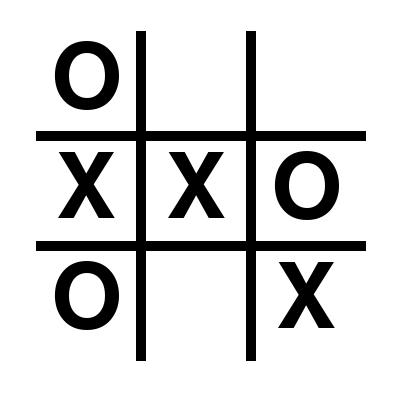
\includegraphics[width=0.2\linewidth,keepaspectratio]{rl70}
\end{center}


\end{frame}

%%%%%%%%%%%%%%%%%%%%%%%%%%%%%%%%%%%%%%%%%%%%%%%%%%%%%%%%%%%%%%%%%%%%%%%%%%%%%%%%%
\begin{frame}[fragile]\frametitle{Min Max Algorithm}


\begin{columns}
\begin{column}{0.5\textwidth}
\begin{itemize}
\item Consider a game which has 4 final states and paths to reach final state are from root to 4 leaves of a perfect binary tree as shown.
\item Assume you are the maximizing player and you get the first chance to move, i.e., you are at the root and your opponent at next level. 
\item Which move you would make as a maximizing player considering that your opponent also plays optimally?
\end{itemize}

\end{column}
\begin{column}{0.5\textwidth}  %%<--- here
\begin{center}
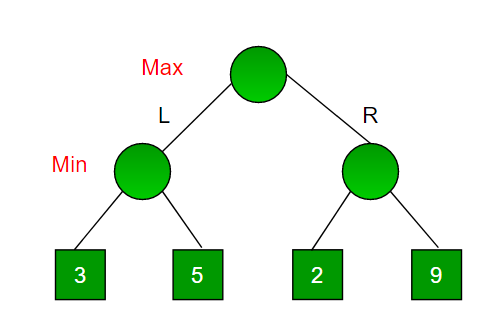
\includegraphics[width=0.8\linewidth,keepaspectratio]{rl71}
\end{center}
\end{column}
\end{columns}

{\tiny (Ref: Minimax Algorithm in Game Theory - Geek For Geeks)}

\end{frame}

%%%%%%%%%%%%%%%%%%%%%%%%%%%%%%%%%%%%%%%%%%%%%%%%%%%%%%%%%%%%%%%%%%%%%%%%%%%%%%%%%
\begin{frame}[fragile]\frametitle{Min Max Algorithm}


\begin{columns}
\begin{column}{0.5\textwidth}
\begin{itemize}
\item This is a backtracking based algorithm, it tries all possible moves, then backtracks and makes a decision. 
\item Maximizer goes LEFT: It is now the minimizers turn. The minimizer now has a choice between 3 and 5. Being the minimizer it will definitely choose the least among both, that is 3
\item Maximizer goes RIGHT: It is now the minimizers turn. The minimizer now has a choice between 2 and 9. He will choose 2 as it is the least among the two values.
\end{itemize}

\end{column}
\begin{column}{0.5\textwidth}  %%<--- here
\begin{center}
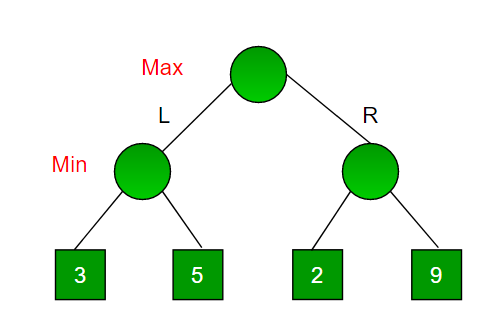
\includegraphics[width=0.8\linewidth,keepaspectratio]{rl71}
\end{center}
\end{column}
\end{columns}

{\tiny (Ref: Minimax Algorithm in Game Theory - Geek For Geeks)}

\end{frame}

%%%%%%%%%%%%%%%%%%%%%%%%%%%%%%%%%%%%%%%%%%%%%%%%%%%%%%%%%%%%%%%%%%%%%%%%%%%%%%%%%
\begin{frame}[fragile]\frametitle{Min Max Algorithm}


\begin{columns}
\begin{column}{0.5\textwidth}
\begin{itemize}
\item Being the maximizer you would choose the larger value that is 3. 
\item Hence the optimal move for the maximizer is to go LEFT and the optimal value is 3.
\end{itemize}

\end{column}
\begin{column}{0.5\textwidth}  %%<--- here
\begin{center}
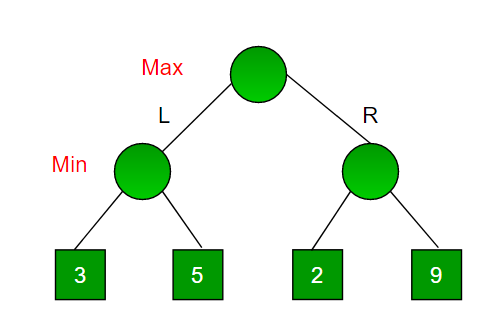
\includegraphics[width=0.8\linewidth,keepaspectratio]{rl71}
\end{center}
\end{column}
\end{columns}

{\tiny (Ref: Minimax Algorithm in Game Theory - Geek For Geeks)}

\end{frame}

%%%%%%%%%%%%%%%%%%%%%%%%%%%%%%%%%%%%%%%%%%%%%%%%%%%%%%%%%%%%%%%%%%%%%%%%%%%%%%%%%
\begin{frame}[fragile]\frametitle{Min Max Tic Tac Toe}


\begin{columns}
\begin{column}{0.5\textwidth}
\begin{itemize}
\item In Tic Tac Toe, in the middle of the games, say, here is the board position
\item Here, of the three possible moves available to player X
\item  ‘X’ in the center square is the only action that leads to a winning outcome
\item Note that Player X makes Move 1, Player Y makes Move 2 and Player X makes Move 3. This mini-game can end as early as after Move 1.
\end{itemize}

\end{column}
\begin{column}{0.5\textwidth}  %%<--- here
\begin{center}
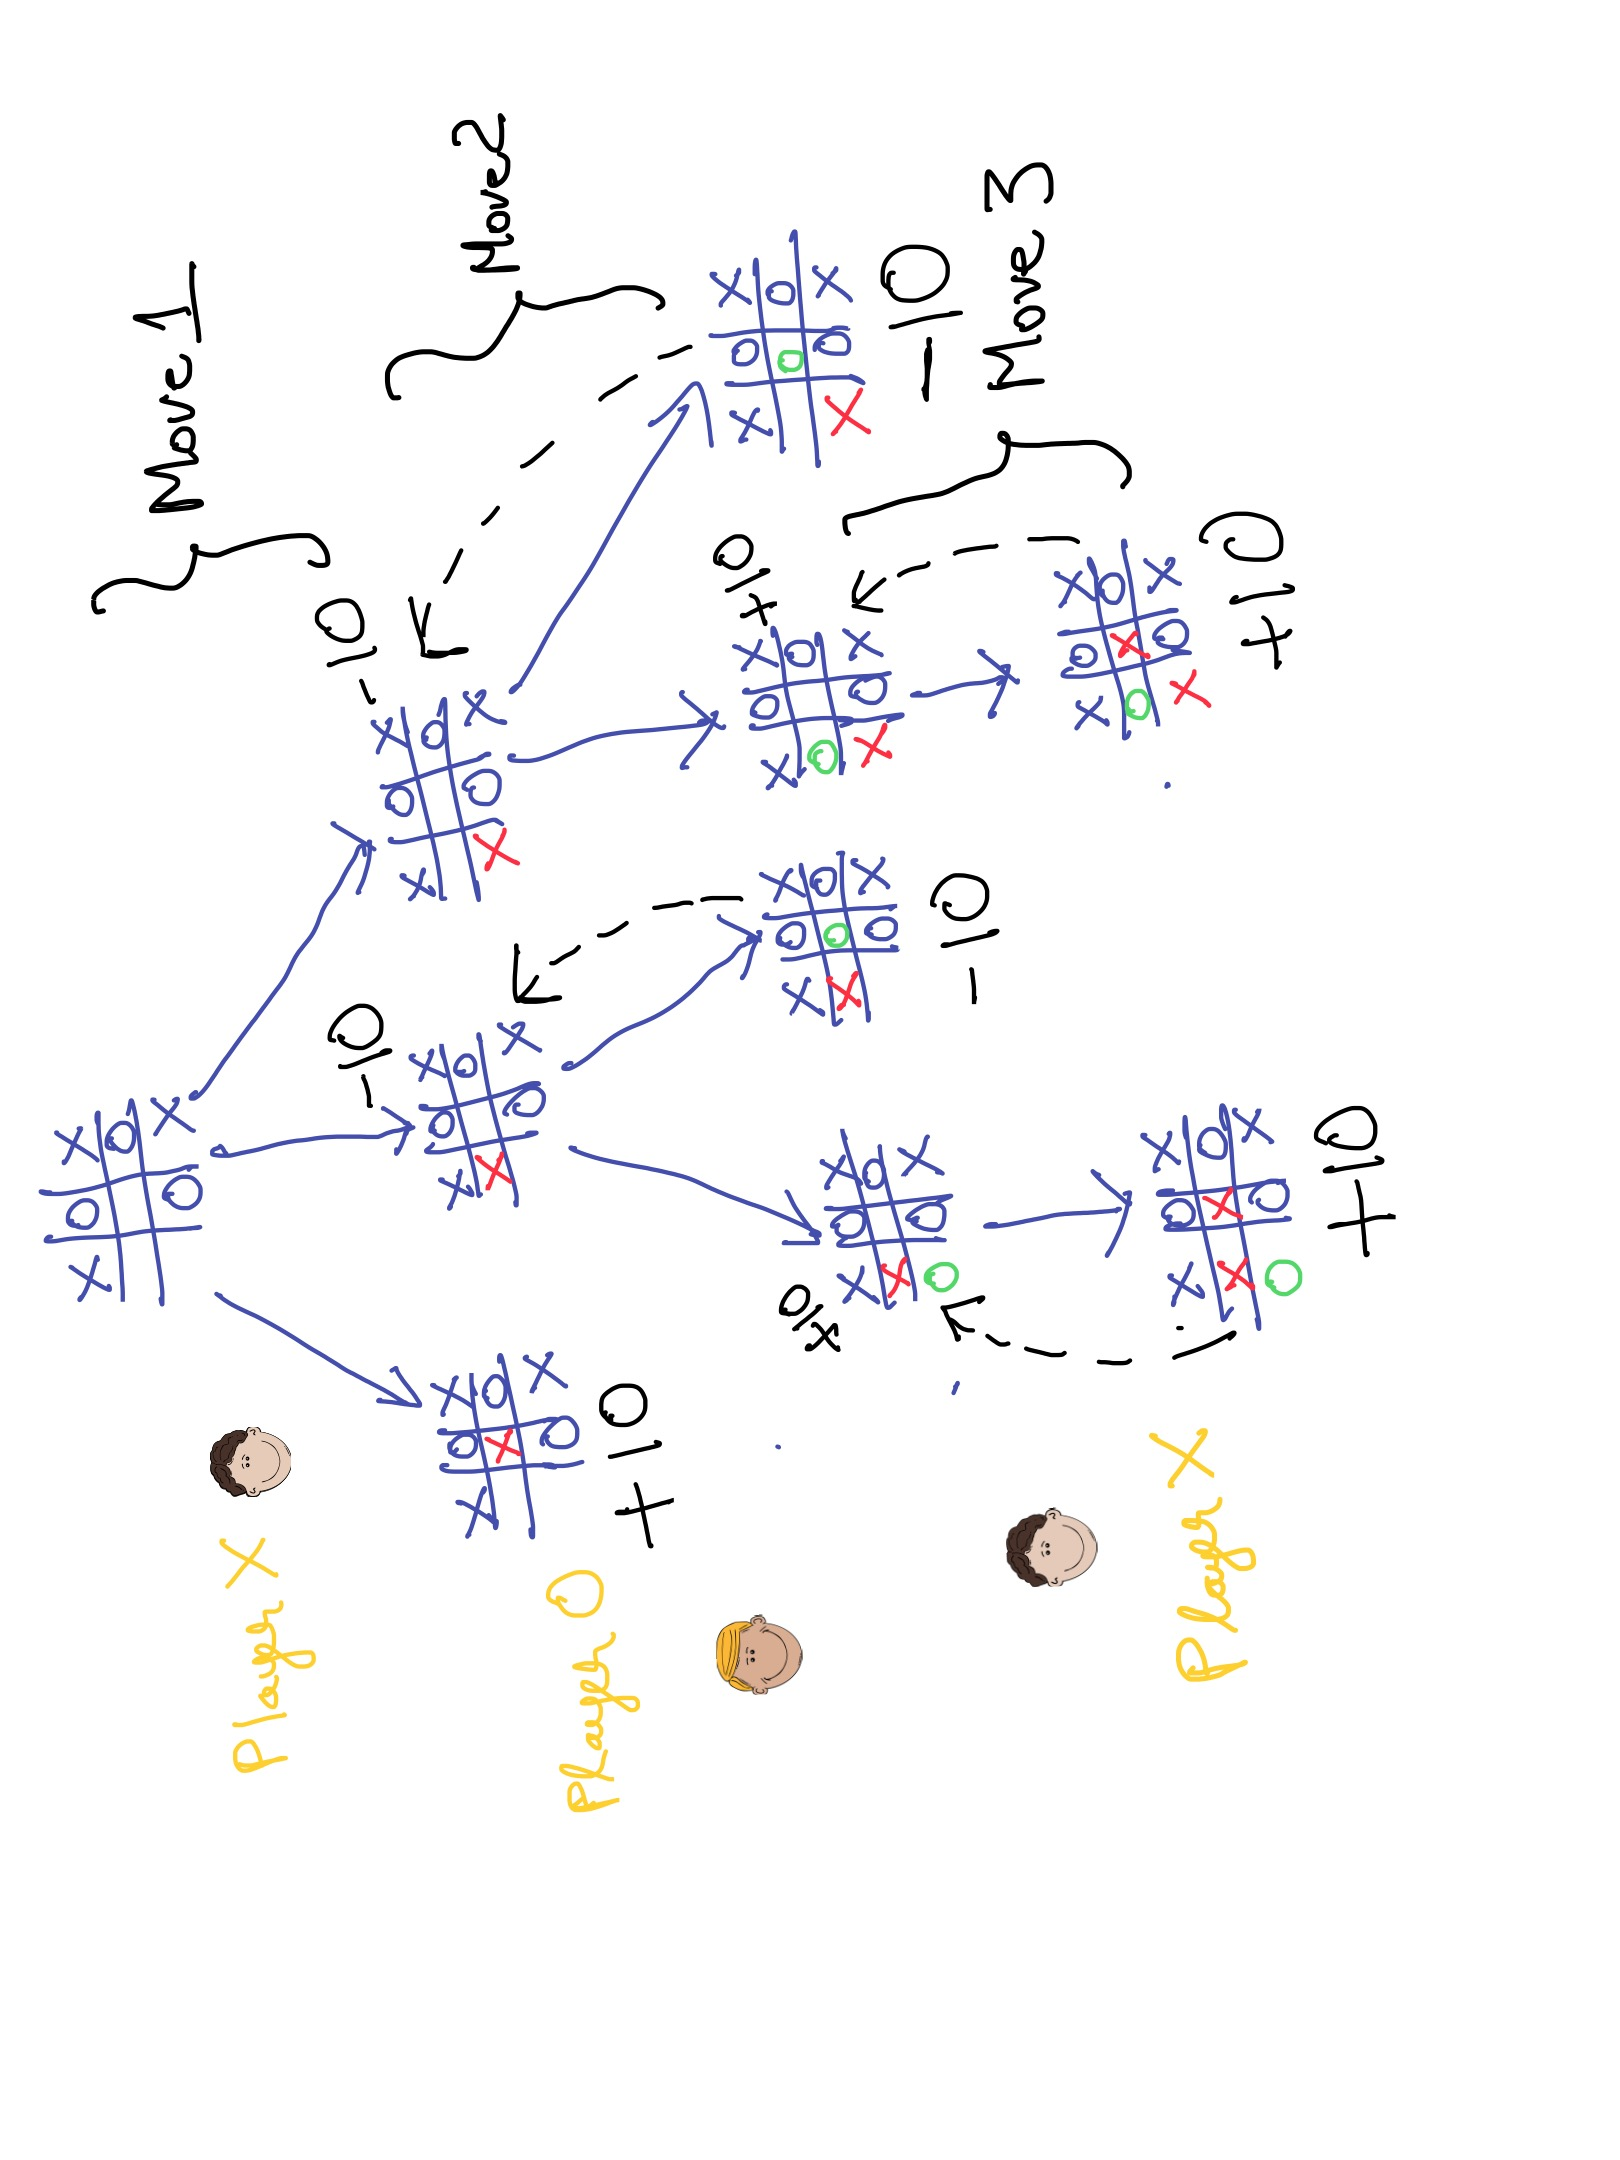
\includegraphics[width=0.8\linewidth,keepaspectratio]{rl72}
\end{center}
\end{column}
\end{columns}

{\tiny (Ref: Solving Tic-Tac-Toe with Minimax - Govind G Nair)}

\end{frame}

%%%%%%%%%%%%%%%%%%%%%%%%%%%%%%%%%%%%%%%%%%%%%%%%%%%%%%%%%%%%%%%%%%%%%%%%%%%%%%%%%
\begin{frame}[fragile]\frametitle{Min Max Tic Tac Toe}



\begin{center}
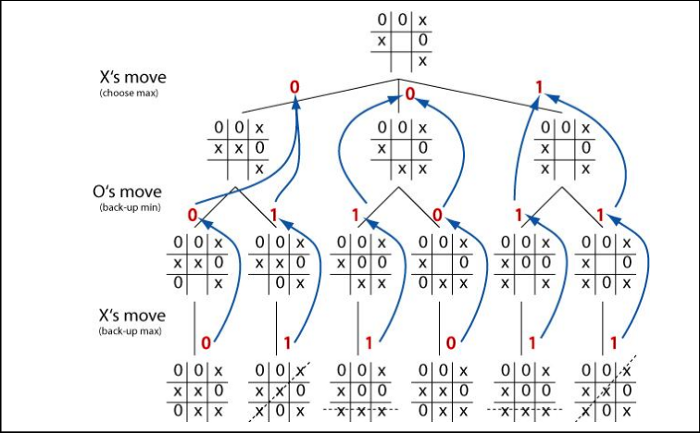
\includegraphics[width=0.8\linewidth,keepaspectratio]{rl74}
\end{center}

Evident that taking move on the right at next level is beneficial.

{\tiny (Ref: Playing Tic Tac Toe using Reinforcement Learning - Rohit Agarwal)}

\end{frame}

%%%%%%%%%%%%%%%%%%%%%%%%%%%%%%%%%%%%%%%%%%%%%%%%%%%%%%%%%%%%%%%%%%%%%%%%%%%%%%%%%
\begin{frame}[fragile]\frametitle{Monte Carlo Tree Search}

\begin{itemize}
\item Monte Carlo Tree Search (MCTS) is powerful RL algorithm, used in AlphaGo, AlphaZero etc.
\item Game Tree: The nodes of a tree represent a state of the game. Edges of a node tell you what possible states can be reached from the current state.
\item A complete game tree contains every possible state of the given game. 
\item If you are able to build a complete game tree then it becomes trivial to calculate which moves are more likely to lead to a win.
\item Suited for low number of possible states and low number of branchings. Cannot work for `Go` as it as $10^{172}$ states, ie more than atoms in the universe ($10^{80}$)
\end{itemize}


\begin{center}
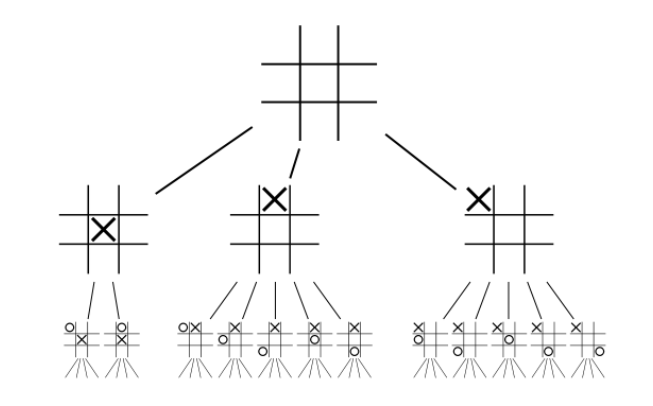
\includegraphics[width=0.4\linewidth,keepaspectratio]{rl82}
\end{center}


{\tiny (Ref: Monte Carlo Tree Search - Deakos Data Science)}

\end{frame}

%%%%%%%%%%%%%%%%%%%%%%%%%%%%%%%%%%%%%%%%%%%%%%%%%%%%%%%%%%%%%%%%%%%%%%%%%%%%%%%%%
\begin{frame}[fragile]\frametitle{Monte Carlo Tree Search}

\begin{itemize}
\item  Each node has two values: $n$ and $w$. 
\item $n$: number of times this state has been considered, 
\item $w$: number of times player won from this position. 
\item Darker nodes: player X has won from that position
\item Lighter nodes: player O has won from that position.
\end{itemize}


\begin{center}
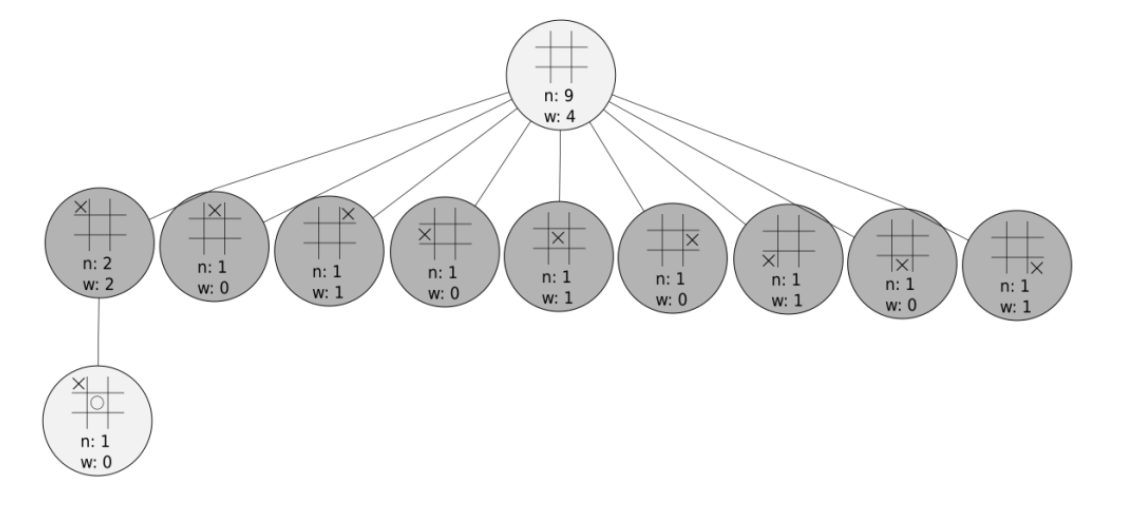
\includegraphics[width=0.8\linewidth,keepaspectratio]{rl83}
\end{center}


{\tiny (Ref: Monte Carlo Tree Search - Deakos Data Science)}

\end{frame}

%%%%%%%%%%%%%%%%%%%%%%%%%%%%%%%%%%%%%%%%%%%%%%%%%%%%%%%%%%%%%%%%%%%%%%%%%%%%%%%%%
\begin{frame}[fragile]\frametitle{Monte Carlo Tree Search}

Possible operations:
\begin{itemize}
\item Selection
\item Expansion
\item Simulation
\item Back-propagation
\end{itemize}

Cycling through these four phases happens during the game.

{\tiny (Ref: Monte Carlo Tree Search - Deakos Data Science)}

\end{frame}

%%%%%%%%%%%%%%%%%%%%%%%%%%%%%%%%%%%%%%%%%%%%%%%%%%%%%%%%%%%%%%%%%%%%%%%%%%%%%%%%%
\begin{frame}[fragile]\frametitle{Selection}

\begin{itemize}
\item To decide which action to take. Max wins or random? (Exploitation vs Exploration). 
\item Combo formula $UCB1 = \frac{w_i}{n_i} + c \sqrt{\frac{\log N}{n_i}}$ where,
	\begin{itemize}
	\item $w_i$: wins considered for that node
	\item $n_i$: number of times that node has been considered (visit count)
	\item $N$: number of times all reachable nodes have been considered (sum of the visit count of all reachable nodes)
	\item $c$: hyper-parameter to choose. Higher for exploration.
	\end{itemize}
\item Say, such $c$ is chosen that following action is suggested. The node we selected doesn’t have any child nodes in the game tree. So, EXPAND.
\end{itemize}

\begin{center}
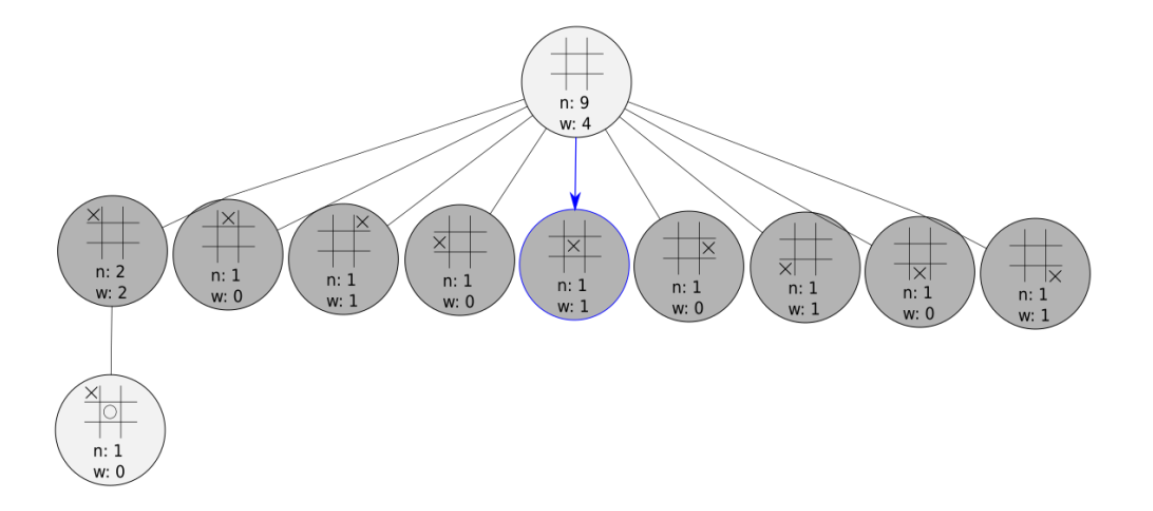
\includegraphics[width=0.7\linewidth,keepaspectratio]{rl84}
\end{center}


{\tiny (Ref: Monte Carlo Tree Search - Deakos Data Science)}

\end{frame}

%%%%%%%%%%%%%%%%%%%%%%%%%%%%%%%%%%%%%%%%%%%%%%%%%%%%%%%%%%%%%%%%%%%%%%%%%%%%%%%%%
\begin{frame}[fragile]\frametitle{Expansion}
Grow our tree!!

\begin{itemize}
\item The opponent has to choose, you can do it randomly (light roll-out) or using some deep algo (deep roll-out).
\item If the game’s not over yet, we move through to the simulation phase. 
\end{itemize}

\begin{center}
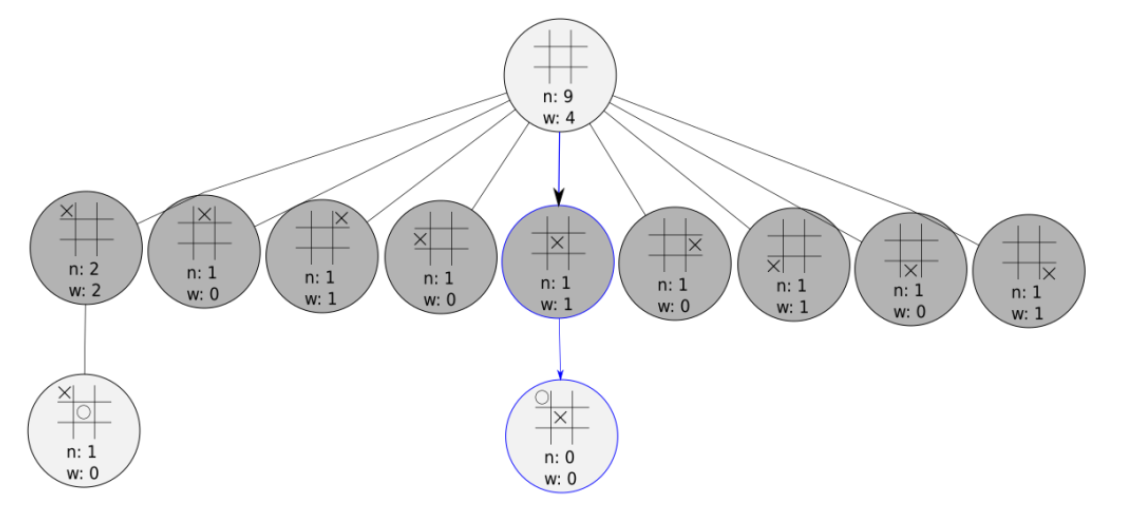
\includegraphics[width=0.8\linewidth,keepaspectratio]{rl85}
\end{center}


{\tiny (Ref: Monte Carlo Tree Search - Deakos Data Science)}

\end{frame}

%%%%%%%%%%%%%%%%%%%%%%%%%%%%%%%%%%%%%%%%%%%%%%%%%%%%%%%%%%%%%%%%%%%%%%%%%%%%%%%%%
\begin{frame}[fragile]\frametitle{Simulation}

\begin{itemize}
\item Simulate the game from our current node to the end and see who won!
\item Simulated out a game and O won it, in this particular path. Time to move to the next phase!
\end{itemize}

\begin{center}
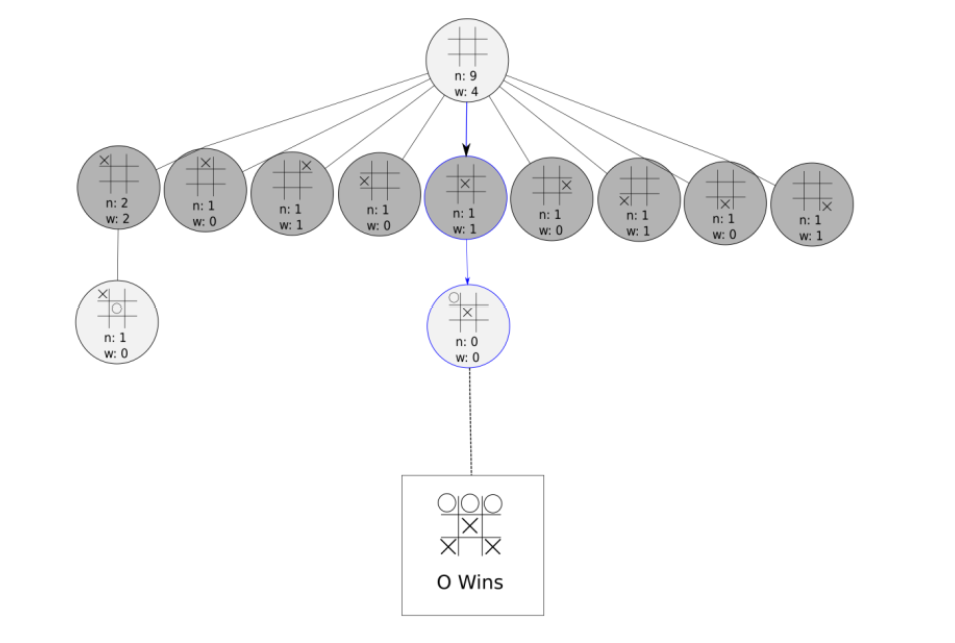
\includegraphics[width=0.8\linewidth,keepaspectratio]{rl86}
\end{center}


{\tiny (Ref: Monte Carlo Tree Search - Deakos Data Science)}

\end{frame}

%%%%%%%%%%%%%%%%%%%%%%%%%%%%%%%%%%%%%%%%%%%%%%%%%%%%%%%%%%%%%%%%%%%%%%%%%%%%%%%%%
\begin{frame}[fragile]\frametitle{Backpropagation}

\begin{itemize}
\item Update our selected nodes with the result of the simulation. 
\item Increment the visit count $n$ in each node, 
\item Update our win count $w$ for only the light gray nodes.
\item Do this hundreds (epochs) of times!!
\end{itemize}

\begin{center}
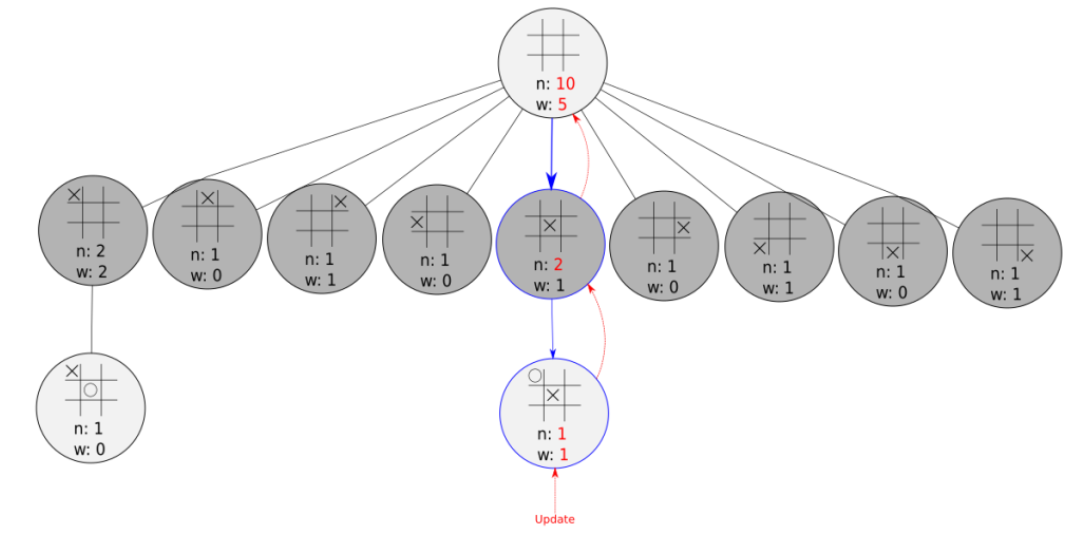
\includegraphics[width=0.8\linewidth,keepaspectratio]{rl87}
\end{center}


{\tiny (Ref: Monte Carlo Tree Search - Deakos Data Science)}

\end{frame}

%%%%%%%%%%%%%%%%%%%%%%%%%%%%%%%%%%%%%%%%%%%%%%%%%%%%%%%%%%%%%%%%%%%%%%%%%%%%%%%%%
\begin{frame}[fragile]\frametitle{Making a move}

\begin{itemize}
\item No move was made yet, just checking which ones look better, right?
\item Once visit and weight counts are done after many epochs, following could be the scene.
\item can pick the action that leads to the node with the highest winning percentage or to the node with the highest visit count
\item Once chosen, repeat the process over and over again until the end of the game.
\end{itemize}

\begin{center}
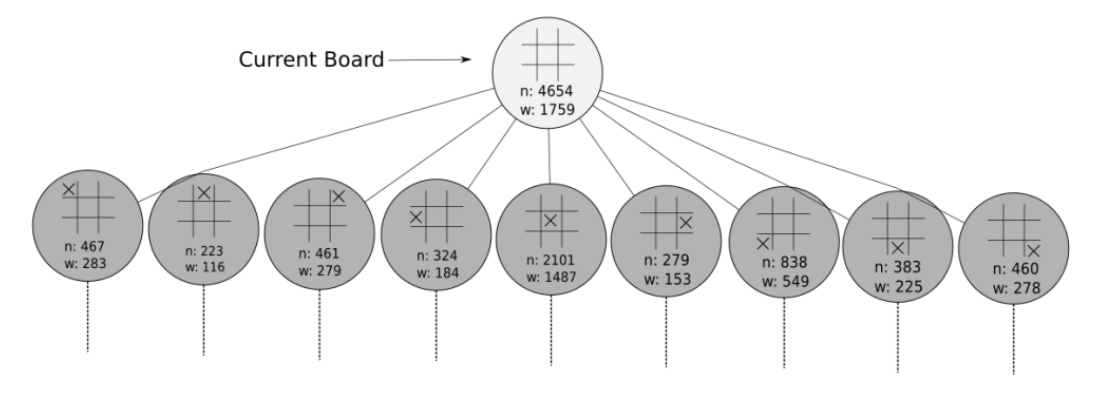
\includegraphics[width=0.8\linewidth,keepaspectratio]{rl88}
\end{center}


{\tiny (Ref: Monte Carlo Tree Search - Deakos Data Science)}

\end{frame}


%%%%%%%%%%%%%%%%%%%%%%%%%%%%%%%%%%%%%%%%%%%%%%%%%%%%%%%%%%%%%%%%%%%%%%%%%%%%%%%%%
\begin{frame}[fragile]\frametitle{MCTS with NN}

\begin{itemize}
\item NN outputs: policy vector and a value
\item policy vector: list of numbers, each number giving the logit probability of choosing a particular action. 
\item value: a real number between -1 and 1 which represents the likelihood that the agent will win from that state. (1 is a win, -1 is a loss and 0 is a draw.)
\item It’s possible use a neural net that just has a policy output, or two different neural nets for policy and value (this was the original AlphaGo design!)
\end{itemize}




{\tiny (Ref: Monte Carlo Tree Search - Deakos Data Science)}

\end{frame}

%%%%%%%%%%%%%%%%%%%%%%%%%%%%%%%%%%%%%%%%%%%%%%%%%%%%%%%%%%%%%%%%%%%%%%%%%%%%%%%%%
\begin{frame}[fragile]\frametitle{MCTS with NN}

\begin{itemize}
\item Instead of a visit count and win count, they will track the visit count $n$, a prior probability $p$, an intermediary value $w$, and an action-value $q$.
\item These are stored on Edges. 
\item Nodes store a ``state value''.
\end{itemize}

\begin{center}
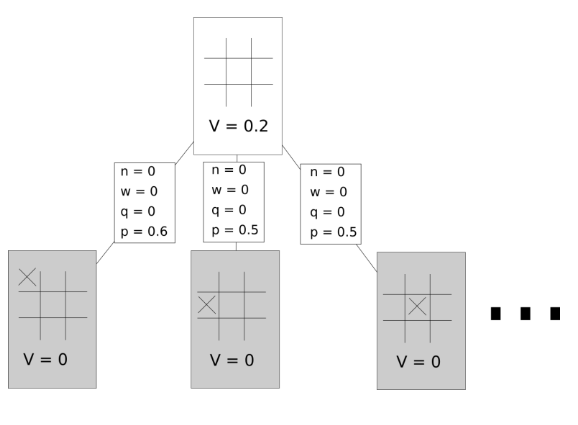
\includegraphics[width=0.6\linewidth,keepaspectratio]{rl89}
\end{center}


{\tiny (Ref: Monte Carlo Tree Search - Deakos Data Science)}

\end{frame}

%%%%%%%%%%%%%%%%%%%%%%%%%%%%%%%%%%%%%%%%%%%%%%%%%%%%%%%%%%%%%%%%%%%%%%%%%%%%%%%%%
\begin{frame}[fragile]\frametitle{Selection}

Selection formula $UCB1$ of vanilla MCTS changes to $Q(s,a) + c P(s,a) \frac{\sqrt{\sum_bN(s,b)}}{1+N(s,a)}$, where, 

\begin{itemize}
\item $N(s,a)$:  visit count of a given game state $s$ and an associated action $a$
\item $P(s,a)$: prior probability of a taking an action from a given game state, predicted by Neural Network.
\item $Q(s,a)$: action-value of a given action at a given state ie represents the value of taking that action
\end{itemize}

Say, by adding Dirichlet noise to our priors, we bring randomness, and thus suggested node is as follows:

\begin{center}
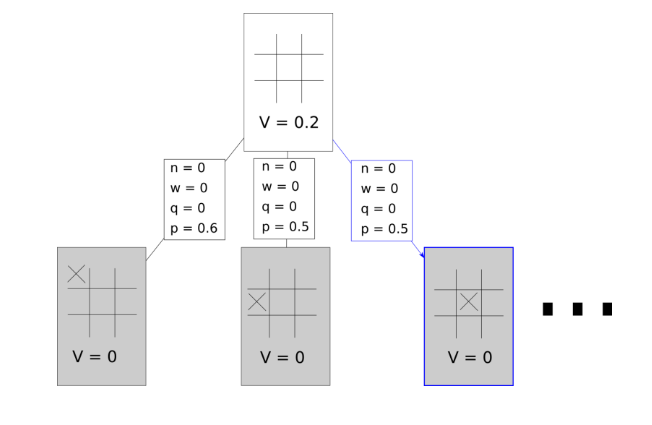
\includegraphics[width=0.4\linewidth,keepaspectratio]{rl90}
\end{center}

{\tiny (Ref: Monte Carlo Tree Search - Deakos Data Science)}

\end{frame}

%%%%%%%%%%%%%%%%%%%%%%%%%%%%%%%%%%%%%%%%%%%%%%%%%%%%%%%%%%%%%%%%%%%%%%%%%%%%%%%%%
\begin{frame}[fragile]\frametitle{Expansion}

\begin{itemize}
\item Neural net has predicted a state value of 0.6
\item Also gives list of nine logit probabilities for our possible nine actions. 
\item These numbers give us the prior probabilities of our edges.
\end{itemize}

\begin{center}
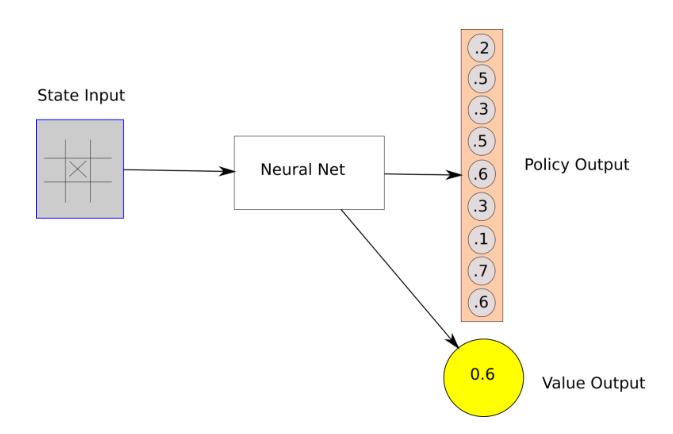
\includegraphics[width=0.8\linewidth,keepaspectratio]{rl91}
\end{center}

{\tiny (Ref: Monte Carlo Tree Search - Deakos Data Science)}

\end{frame}

%%%%%%%%%%%%%%%%%%%%%%%%%%%%%%%%%%%%%%%%%%%%%%%%%%%%%%%%%%%%%%%%%%%%%%%%%%%%%%%%%
\begin{frame}[fragile]\frametitle{Expanded}

\begin{center}
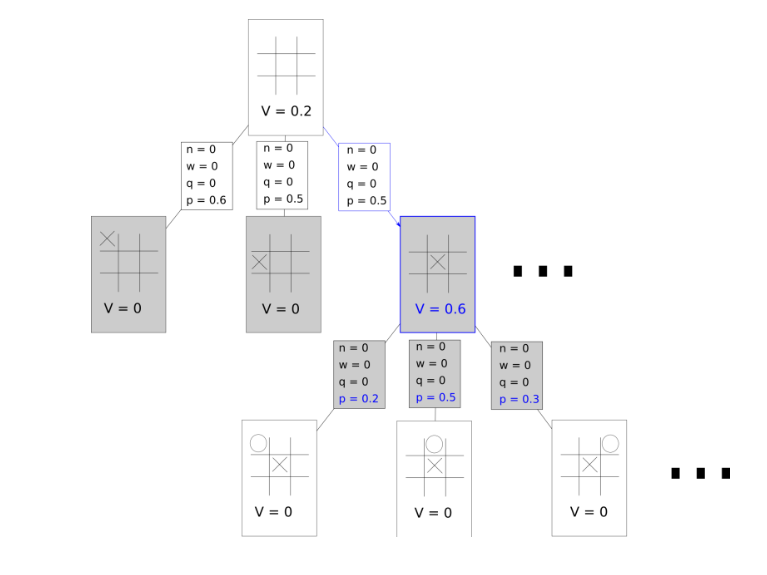
\includegraphics[width=0.8\linewidth,keepaspectratio]{rl92}
\end{center}

{\tiny (Ref: Monte Carlo Tree Search - Deakos Data Science)}

\end{frame}

%%%%%%%%%%%%%%%%%%%%%%%%%%%%%%%%%%%%%%%%%%%%%%%%%%%%%%%%%%%%%%%%%%%%%%%%%%%%%%%%%
\begin{frame}[fragile]\frametitle{Updated}

For every edge $e_t$ that was traversed up until the recently expanded leaf node, three updates are performed.

\begin{itemize}
\item The visit count is incremented.
\item If the player that owns $e_t$ is the same player that owns the leaf node, then we add $v$ to $w$. Otherwise, we subtract $v$ from $w$.
\item We update the action-value $q$ to $w/n$.
\end{itemize}

\begin{center}
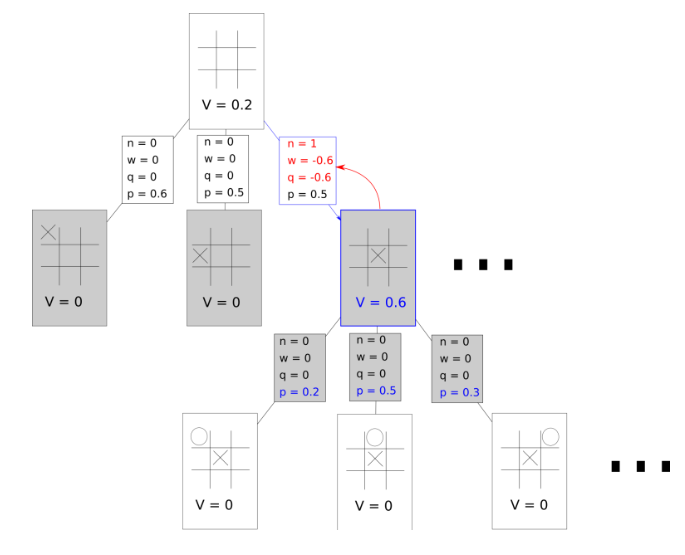
\includegraphics[width=0.5\linewidth,keepaspectratio]{rl93}
\end{center}

{\tiny (Ref: Monte Carlo Tree Search - Deakos Data Science)}

\end{frame}

%%%%%%%%%%%%%%%%%%%%%%%%%%%%%%%%%%%%%%%%%%%%%%%%%%%%%%%%%%%%%%%%%%%%%%%%%%%%%%%%%
\begin{frame}[fragile]\frametitle{Repeat!}

Process is repeated till all epochs are done. Here are the steps:

Expand till leaf node


\begin{center}
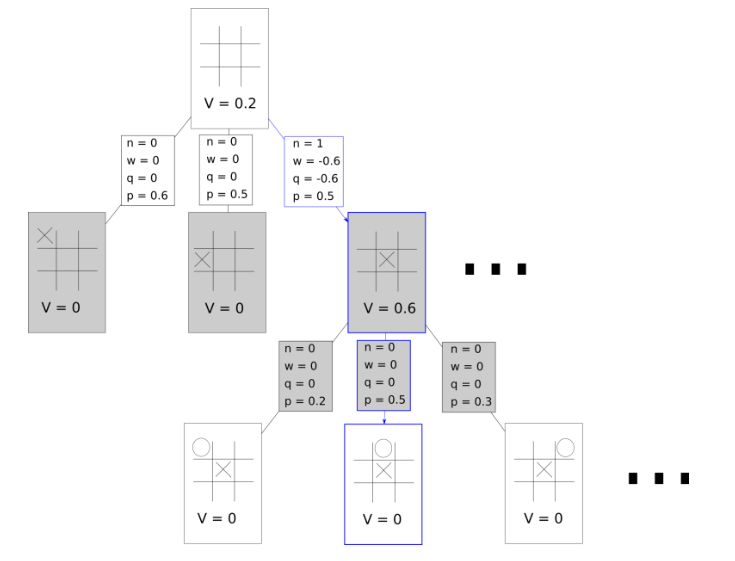
\includegraphics[width=0.6\linewidth,keepaspectratio]{rl94}
\end{center}

{\tiny (Ref: Monte Carlo Tree Search - Deakos Data Science)}

\end{frame}

%%%%%%%%%%%%%%%%%%%%%%%%%%%%%%%%%%%%%%%%%%%%%%%%%%%%%%%%%%%%%%%%%%%%%%%%%%%%%%%%%
\begin{frame}[fragile]\frametitle{Repeat!}

Expand and Evaluate the Leaf Node

\begin{center}
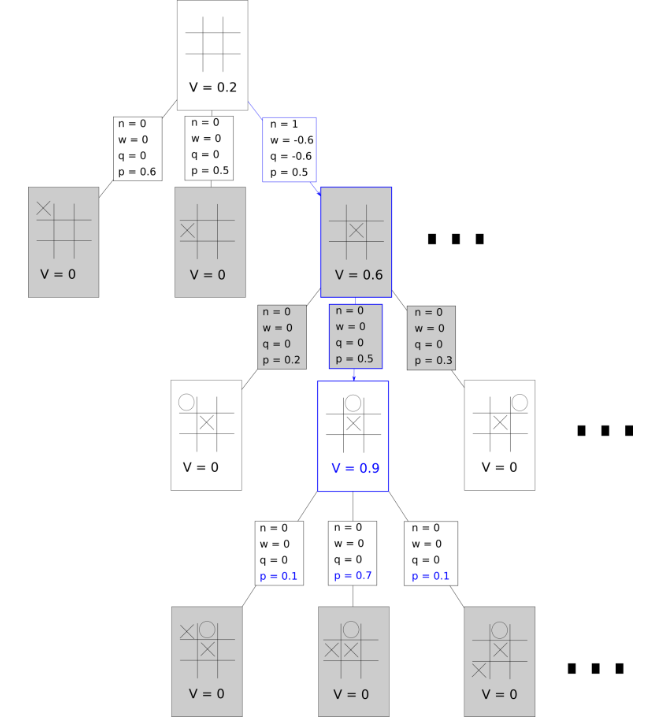
\includegraphics[width=0.5\linewidth,keepaspectratio]{rl95}
\end{center}

{\tiny (Ref: Monte Carlo Tree Search - Deakos Data Science)}

\end{frame}

%%%%%%%%%%%%%%%%%%%%%%%%%%%%%%%%%%%%%%%%%%%%%%%%%%%%%%%%%%%%%%%%%%%%%%%%%%%%%%%%%
\begin{frame}[fragile]\frametitle{Repeat!}

Update All Traversed Edges according to the value of the leaf node.

\begin{center}
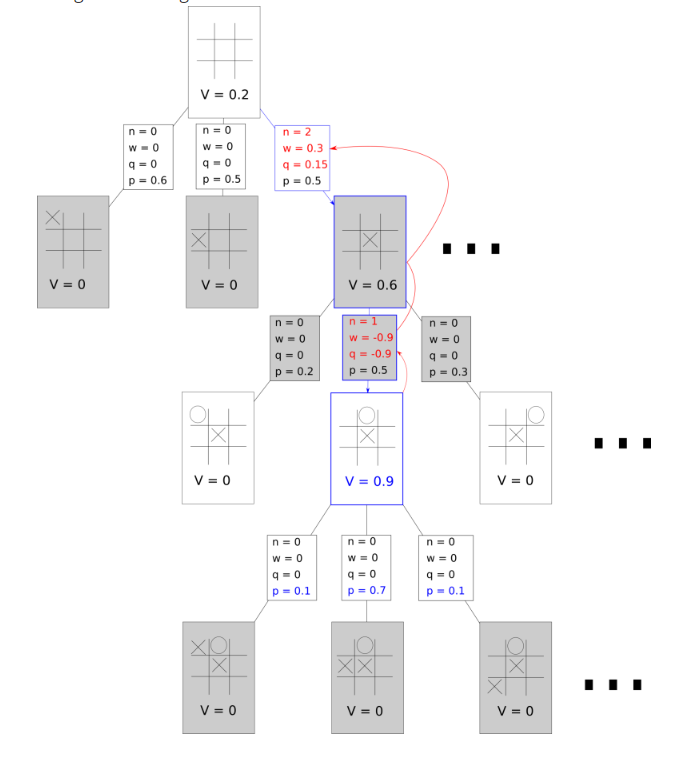
\includegraphics[width=0.5\linewidth,keepaspectratio]{rl96}
\end{center}

{\tiny (Ref: Monte Carlo Tree Search - Deakos Data Science)}

\end{frame}


%%%%%%%%%%%%%%%%%%%%%%%%%%%%%%%%%%%%%%%%%%%%%%%%%%%%%%%%%%%%%%%%%%%%%%%%%%%%%%%%%
\begin{frame}[fragile]\frametitle{Choosing an Action}

\begin{itemize}
\item After the steps above have been repeated many times, we’ll have a pretty big game tree. 
\item Now choose which move we actually want to play! 
\item We generate a list of probabilities of choosing a given action according to this formula $\pi_t = N(s,s)^{1/t}/\sum_b N(s,b)^{1/t}$
\item The temperature parameter $t$ describes how much you want to value the visit count of a given edge. 
\item The closer to zero this is set, the more chance there is of choosing greedily with respect to visit count, where a temperature parameter of one will more readily choose less-explored actions.
\end{itemize}


{\tiny (Ref: Monte Carlo Tree Search - Deakos Data Science)}

\end{frame}


%%%%%%%%%%%%%%%%%%%%%%%%%%%%%%%%%%%%%%%%%%%%%%%%%%%%%%%%%%%%%%%%%%%%%%%%%%%%%%%%%
\begin{frame}[fragile]\frametitle{Using MCTS Results as Training Data}

\begin{columns}
\begin{column}{0.5\textwidth}
\begin{itemize}
\item How do we make sure the neural net keeps improving with constant play? 
\item After playing an entire game against itself using MCTS, we generate some data-points.
\item Each move we’ve played has an input state, a target value (depending on who won), a predicted value, a predicted policy (the prior probabilities of each edge), and a target policy (the search probabilities of each edge). 
\item This is all we need to train our neural net.
\end{itemize}
\end{column}
\begin{column}{0.5\textwidth}
\begin{center}
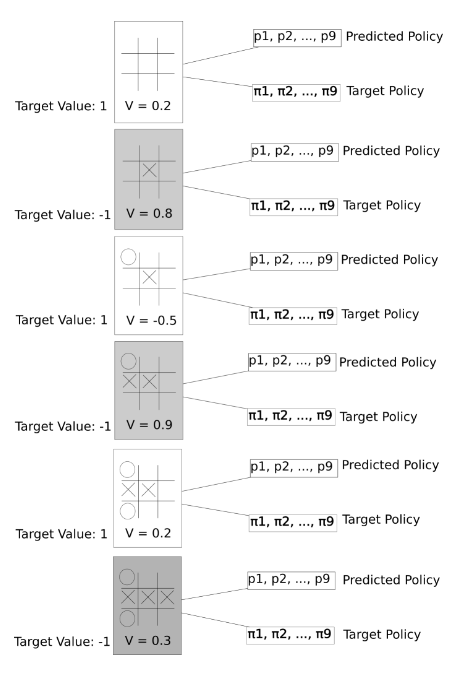
\includegraphics[width=0.8\linewidth,keepaspectratio]{rl97}
\end{center}
\end{column}
\end{columns}



{\tiny (Ref: Monte Carlo Tree Search - Deakos Data Science)}

\end{frame}

%%%%%%%%%%%%%%%%%%%%%%%%%%%%%%%%%%%%%%%%%%%%%%%%%%%%%%%%%%%%%%%%%%%%%%%%%%%%%%%%%
\begin{frame}[fragile]\frametitle{Important Note}

\begin{itemize}
\item We shouldn’t be constantly training the neural network that’s guiding our MCTS and generating our data. 
\item Instead, we have two neural networks – our data generation network and our training network. 
\item The data generation network is what we actually use in our MCTS simulations. 
\item This network generates new data for the training network to learn from. 
\item After a set number of training steps (1000 for AlphaGo Zero), an MCTS using our training network is pitted against one with our data generation network in a tournament. 
\item If the data generation network loses, it gets replaced by our training network.
\end{itemize}


{\tiny (Ref: Monte Carlo Tree Search - Deakos Data Science)}

\end{frame}





